% TEMPLATE for Usenix papers, specifically to meet requirements of
%  USENIX '05
% originally a template for producing IEEE-format articles using LaTeX.
%   written by Matthew Ward, CS Department, Worcester Polytechnic Institute.
% adapted by David Beazley for his excellent SWIG paper in Proceedings,
%   Tcl 96
% turned into a smartass generic template by De Clarke, with thanks to
%   both the above pioneers
% use at your own risk.  Complaints to /dev/null.
% make it two column with no page numbering, default is 10 point

% Munged by Fred Douglis <douglis@research.att.com> 10/97 to separate
% the .sty file from the LaTeX source template, so that people can
% more easily include the .sty file into an existing document.  Also
% changed to more closely follow the style guidelines as represented
% by the Word sample file. 

% Note that since 2010, USENIX does not require endnotes. If you want
% foot of page notes, don't include the endnotes package in the 
% usepackage command, below.

% This version uses the latex2e styles, not the very ancient 2.09 stuff.
\documentclass[letterpaper,twocolumn,10pt]{article}
\usepackage{usenix,epsfig,endnotes}
\usepackage{cite}
\usepackage{amsmath,amssymb,amsfonts}
\usepackage{algorithmic}
\usepackage{graphicx}
\usepackage{textcomp}
\usepackage{amsfonts,amsthm,amsmath,amssymb}
\usepackage{hyperref}
\usepackage{framed}
\usepackage{array}
\usepackage{epsfig}
\usepackage{tikz}
\usepackage{enumitem} 
\usepackage{url}
\usepackage{graphicx}
\usepackage{pgfplotstable}
\usepackage{pgfplots} 
\usetikzlibrary{positioning}
\def\BibTeX{{\rm B\kern-.05em{\sc i\kern-.025em b}\kern-.08em
    T\kern-.1667em\lower.7ex\hbox{E}\kern-.125emX}}
    
\newcommand{\ignore}[1]{}

\newtheorem{theorem}{Theorem}
\newtheorem{definition}[theorem]{Definition}
\newcommand{\getsR}{\overset{\$}{\leftarrow}}  
\def\name/{ObliDB}

\pgfplotsset{width=6cm,compat=1.9} 

% Alter some LaTeX defaults for better treatment of figures:
    % See p.105 of "TeX Unbound" for suggested values.
    % See pp. 199-200 of Lamport's "LaTeX" book for details.
    %   General parameters, for ALL pages:
    \renewcommand{\topfraction}{0.9}	% max fraction of floats at top
    \renewcommand{\bottomfraction}{0.8}	% max fraction of floats at bottom
    %   Parameters for TEXT pages (not float pages):
    \setcounter{topnumber}{2}
    \setcounter{bottomnumber}{2}
    \setcounter{totalnumber}{4}     % 2 may work better
    \setcounter{dbltopnumber}{2}    % for 2-column pages
    \renewcommand{\dbltopfraction}{0.9}	% fit big float above 2-col. text
    \renewcommand{\textfraction}{0.07}	% allow minimal text w. figs
    %   Parameters for FLOAT pages (not text pages):
    \renewcommand{\floatpagefraction}{0.9}	% require fuller float pages
	% N.B.: floatpagefraction MUST be less than topfraction !!
    \renewcommand{\dblfloatpagefraction}{0.9}	% require fuller float pages

	% remember to use [htp] or [htpb] for placement
\begin{document}

%don't want date printed
\date{}

%make title bold and 14 pt font (Latex default is non-bold, 16 pt)
\title{\Large \bf \name/: A Protected Database with Near-Minimal Leakage Using SGX}

\ignore{
%for single author (just remove % characters)
\author{
{\rm Your N.\ Here}\\
Your Institution
\and
{\rm Second Name}\\
Second Institution
% copy the following lines to add more authors
% \and
% {\rm Name}\\
%Name Institution
} % end author
}
\maketitle

% Use the following at camera-ready time to suppress page numbers.
% Comment it out when you first submit the paper for review.
\thispagestyle{empty}

 
\subsection*{Abstract}
Applications meant to handle private data using Intel SGX often leak private information through access patterns to data stored outside the SGX enclave. Access patterns can be naively hidden by using an ORAM and directly porting various SQL operators to their oblivious counterparts, but this approach suffers from unacceptable performance loss. The challenge of oblivious SGX system design, then, lies in developing oblivious algorithms, with or without ORAM, that retain performance near to that of their non-oblivious counterparts. 

We present \name/, a database built on Intel's SGX hardware that provides minimal leakage of cryptographically protected data. \name/ achieves superior performance to prior work while leaking only the structure of queries and the protected data returned from them. In particular, \name/ hides access patterns to data. \name/ supports a broad range of SQL queries including groupings and joins and makes use of both ORAM-based oblivious indexes and linear search-based data structures. It also provides a range of oblivious algorithms to execute operators with different selectivity. 

We evaluate \name/ on several real-world data sets and queries, finding that \name/ outperforms a baseline implementation by 9-500$\times$ and Opaque's oblivious mode~\cite{ZDB+17} by 1.2-20$\times$, coming within 2.1$\times$ of the performance of Spark SQL\cite{SparkSQL}, a system with no data privacy guarantees.  

\section{Introduction}

The advent of cloud computing has ushered in hopes of a future where data owners can outsource their databases while retaining data security. In recent years, a smorgasbord of solutions to the problems of cryptographically-protected databases and search over encrypted data has explored a large space of tradeoffs between performance and leakage of private queries and data~\cite{FVY+17}, but performant systems which provide the highest levels of security -- that of hiding even access patterns to protected data -- remain out of reach. Meanwhile, increasing interest in trusted hardware solutions, lent impetus by the appearance of Intel's SGX~\cite{CD16} has allowed for dramatic speedups in tasks previously requiring heavy and slow cryptographic operations~\cite{FVBG16, NFR+17}. While SGX alone partially solves the problem of protected databases~\cite{FBB+17}, preventing leakage of data access patterns requires more work. Several prior works~\cite{PBP16, DPP+16, FVY+17} mention the possibility of generically using Oblivious RAM (ORAM) on top of SGX to hide these access patterns but point out that, unfortunately, simply running a generic database application over ORAM adds significant slowdowns.

We present \name/, an SGX-based system that specializes data structures and query execution for the database case and leaks only structural information about queries, results, and stored data -- the leakage that can be hidden only by padding. \name/ provides both indexed and unindexed tables and supports many SQL queries including the aggregates \texttt{COUNT}, \texttt{SUM}, \texttt{MIN}, \texttt{MAX}, and \texttt{AVG}, as well as \texttt{SELECT}, \texttt{INSERT}, \texttt{UPDATE}, \texttt{DELETE}, \texttt{GROUP BY} and \texttt{JOIN} queries, a broader set of queries than those supported by most systems offering search over encrypted data that hide data access patterns~\cite{FVY+17}. \name/ also supplies a number of algorithms that optimize operator performance based on the size of data to be returned from a query, thereby providing better performance without any additional leakage. 

We implement a prototype of \name/ and report on its performance, testing it with microbenchmarks on synthetic data of up to 500,000 rows and real queries on multiple real-world data sets of various sizes: domestic US flight data~\cite{FLIGHT}, consumer complaints to the consumer financial protection bureau~\cite{CFPB}, the NASDAQ stock exchange~\cite{NASDAQ}, and the tables and queries of the Big Data Benchmark~\cite{BDB}. We compare \name/ to a baseline implementation where a database index is generically modified to provide data access obliviousness via ORAM and show that \name/ outperforms the baseline by 4.5$\times$ and 1.2$\times$ on insertions and deletions, respectively, and by 9-499$\times$ on realistic queries to data. We also compare \name/ to prior work and find that \name/ performs comparably to the range search scheme of Demertzis et al~\cite{DPP+16} which does not hide access patterns and ranges from 1.2-20$\times$ faster than Opaque's Oblivious mode~\cite{ZDB+17}, an SGX-based data analytics platform that does hide access patterns, suggesting that \name/ and Opaque are fundamentally well-suited to different use cases. Moreover, \name/ comes within at least 2.1$\times$ of the performance of Spark SQL~\cite{SparkSQL}, which provides no security or privacy guarantees, on all implemented Big Data Benchmark queries. Finally, we show that the choices of oblivious data structures and algorithms available in \name/ allow for meaningful optimizations in different data and query settings. 

The rest of this paper is organized as follows: Section~\ref{model} gives an overview of \name/ and the security model in which we operate. Section~\ref{background} gives background on relevant tools used in \name/, and Sections~\ref{oblivData} and~\ref{oblivOps} detail \name/'s design. Sections~\ref{imp} and~\ref{eval} describe our implementation and evaluation respectively, and Section~\ref{related} discusses related work before concluding in Section~\ref{conclusion}. 

\section{Overview}\label{model}
This section summarizes the functionality and architecture of \name/, its threat model, and the security properties it achieves. 

\subsection{Threat Model}
We assume a malicious operating system (OS) with power to examine and modify untrusted memory and any communication between the processor and memory. Moreover, the OS can observe access patterns to trusted memory and maliciously schedule processes or interrupt the execution of an enclave. We note that a malicious OS can always launch an indefinite denial of service attack against an enclave, but such an attack does not compromise privacy and lies outside the scope of the security of the hardware enclave for our purposes. 

We assume security of the SGX platform in that the enclave hides the contents of protected memory pages from a malicious OS, and we do not directly handle side-channels known to affect SGX hardware such as page fault timing attacks~\cite{XCP15} and branch shadowing~\cite{LSG+16}. General solutions exist to protect against such side channels and are compatible with \name/ (see Section~\ref{related} for an overview). 

Furthermore, we also assume a secure channel exists through which an outside user can send messages to the enclave. \ignore{ (this is fairly straightforward with SGX), but we did not implement this for our tests, as it is not directly related to the functionality provided by \name/.} 
 
\subsection{Security Goals}
Queries in \name/ leak only the sizes of tables involved, including intermediate tables, and the query plan used. This includes the sizes of tables in the database, the sizes of queries, and the sizes of responses to queries and provides the same level of security as Opaque's Oblivious Mode~\cite{ZDB+17}. \name/ additionally has a padding mode where sizes of all tables are padded to some chosen size. Further details regarding how to achieve these leakage properties appear in Sections~\ref{oblivData} and~\ref{oblivOps}, where the leakage of each operator is explained. Data at rest outside the enclave is encrypted and MACed and leaks only the size of the encrypted data. We do not make an effort to hide the number of tables in a database or which table(s) a particular query accesses. Our goals deal only with the security of data within individual tables.

We additionally make the integrity guarantee that \name/ catches and reports any tampering with data by the malicious OS. We use a series of checks and safeguards to protect against arbitrary tampering within rows of a table, addition/removal of rows, shuffling of the contents of a table, or rollbacks to a previous system state. We discuss these protections in Section~\ref{oblivData}.

We remark that however secure the properties of a database management system, an application interacting with it can leak additional information. For example, if a web application makes a second query to a database based on the results of a first query, observing the size of the response to the second query may leak additional information about the first query or its response. This direct, if unexpected, consequence of size leakage requires that application developers consider performance goals against the ramifications of such leakage in their design process. 

\subsection{\name/ Architecture Overview}
\begin{figure}
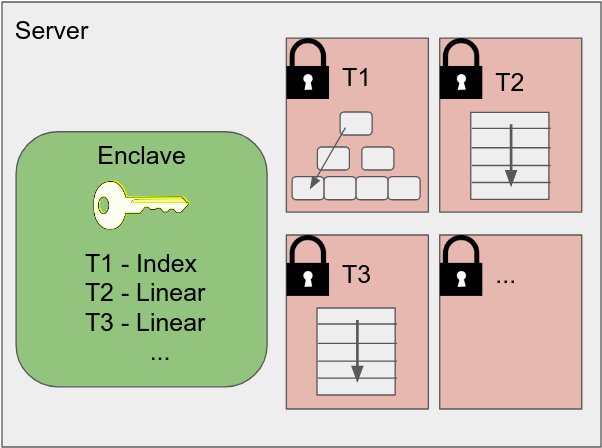
\includegraphics[width=\linewidth]{figure_server.png}
\caption{\name/ provides an interface to a secure enclave with control over encrypted tables stored in untrusted memory. It stores tables either as an oblivious index or a linear scan data structure to ensure data-oblivious queries.}
\label{arch}
\end{figure}
\name/ consists of a trusted code base inside an SGX enclave that provides an interface for users to create, modify, and query tables. \name/ supports tables both with and without indexes, called Indexed and Linear tables, respectively. It stores tables, encrypted, in unprotected memory and obliviously accesses them as needed by the various supported operators. Indexed tables consist of an ORAM with a B+ tree stored inside, whereas Linear tables rely on accessing every block of the underlying data structure to ensure obliviousness. This overview of \name/'s architecture is summarized in Figure~\ref{arch}.

  \name/ supports oblivious versions of the SQL operators \texttt{SELECT}, \texttt{INSERT}, \texttt{UPDATE}, \texttt{DELETE}, \texttt{GROUP BY} and \texttt{JOIN} as well as the aggregates \texttt{COUNT}, \texttt{SUM}, \texttt{MIN}, \texttt{MAX}, and \texttt{AVG}. Each operator is implemented for both Linear and Indexed tables. Additionally, we include several different algorithms for the \texttt{SELECT} and \texttt{GROUP BY} operators, each of which performs better for a different output table size. Our \texttt{SELECT} implementation begins by scanning the table being queried to determine which algorithm to use and then executing the appropriate choice for the expected output size. 

\section{Background}\label{background}
In this section we give a basic overview of Intel SGX and ORAM, the primary tools used in \name/, providing only sufficient detail for the subsequent sections. For more information on work using these primitives, particularly applications, attacks, and defenses for SGX, see Section~\ref{related}.

\subsection{Intel SGX}

SGX provides developers with the abstraction of a secure \textit{enclave} which can verifiably run a trusted code base (TCB) and protects its limited memory from a malicious or compromised OS \cite{CD16, SGXRef}. SGX handles the process of entering and exiting an enclave and hiding the activity of the enclave while non-enclave code runs, albeit imperfectly~\cite{LSG+16}. Enclave code invariably requires access to OS resources, so SGX provides an interface between the enclave and the OS based on \textit{OCALLs} and \textit{ECALLs}. OCALLs are calls made from inside the enclave to the OS, usually for procedures requiring resources managed by the OS, such as access to files on disk. ECALLs allow code outside the TCB to call the enclave to execute trusted code. 

SGX proves that the code running in an enclave is an untampered version of the desired code through a mechanism named \textit{attestation}. Attestation involves an enclave providing a hash of its initial state which a client compares with the expected value of the hash and rejects if there is any evidence of a corrupted or altered program. 

The most significant feature of SGX for our purposes concerns the protection of memory. SGX provides the developer with approximately 90MB of Enclave Page Cache (EPC), a memory region hidden from the OS and cleared whenever execution enters or exits an enclave. In this memory, the enclave can execute trusted code and keep secrets from a malicious OS who otherwise controls the machine executing the code. 

\subsection{ORAM}
Oblivious RAM, or ORAM, is a cryptographic primitive first proposed by Goldreich and Ostrovsky~\cite{GO96} that hides access patterns to data in untrusted memory. In the traditional ORAM setting, a small trusted processor uses a larger memory over a bus on which an adversary may examine communications. Merely encrypting the data that travels over the bus still reveals the access patterns to the data being requested and can be used to glean private information about the data or the queries on it~\cite{IKK12}. ORAM goes further and shuffles the locations of blocks in memory so repeated accesses to the same block and other patterns are hidden from the observing adversary. ORAMs guarantee that any two sets of access patterns of the same length are indistinguishable from each other. More formally, the security of ORAM is defined as follows:
\begin{definition}[ORAM Security\cite{SDS+13}]
Let $\overrightarrow{y}:=\textbf{((op$_M$, a$_M$, data$_M$),...,(op$_1$, a$_1$, data$_1$))}$ denote a data request sequence of length $M$, where each \textbf{op$_i$} denotes a \textbf{read(a$_i$)} or a \textbf{write(a$_i$, data)} operation. Specifically, \textbf{a$_i$} denotes the identifier of the block being read or written, and \textbf{data$_i$} denotes the data being written. Index $1$ corresponds to the most recent load/store and index $M$ corresponds to the oldest load/store operation. 

Let $A(\overrightarrow{y})$ denote the (possibly randomized) sequence of accesses to the untrusted storage given the sequence of data requests $\overrightarrow{y}$. An ORAM construction is said to be secure if:
\begin{enumerate}
\setlength\itemsep{0pt}
\item For any two data request sequences $\overrightarrow{y}$ and $\overrightarrow{z}$ of the the same length, their access patterns $A(\overrightarrow{y})$ and $A(\overrightarrow{z})$ are computationally indistinguishable by anyone but the client ORAM controller.

\item The ORAM construction is correct in the sense that it returns on input $\overrightarrow{y}$ data that is consistent with $\overrightarrow{y}$ with probability $\geq 1 - \textit{negl}(|\overrightarrow{y}|)$, i.e., the ORAM may fail with probability $\textit{negl}(|\overrightarrow{y}|)$.
\end{enumerate}
\end{definition}

The scope of the security guarantees provided by ORAM create important consequences for oblivious data structures and algorithms built on top of ORAM. ORAM only makes guarantees of indistinguishability for access patterns of the same length. This means that oblivious algorithms using ORAM must always make the same number of memory accesses or risk leaking access pattern data.

Although other, older schemes have recently received attention due their practical efficiency in certain practical parameter settings~\cite{ZWR+16}, the most efficient ORAM scheme known is the Path ORAM~\cite{SDS+13}. Path ORAM belongs to a family of schemes known as tree-based ORAMs, which operate by storing the blocks of the oblivious memory in a tree structure. Each block is associated with a leaf in the tree in a position map that guarantees the block will be found somewhere on the path to that leaf. An access to the ORAM involves reading a path down the tree from the root to the leaf corresponding to the desired block. After retrieving the desired block, a second pass is made on the same path where each block is re-encrypted with new randomness and the retrieved block is assigned a new leaf, remaining stored in a small ``stash'' if the path does not allow space for it to be written back on the path to its new assigned leaf. Although it is not always necessary in practice, the position map holding the assigned leaves for each block of the ORAM can be recursively stored in its own ORAM to reduce the trusted processor memory required by this scheme to a constant.

\ignore{
\subsection{B+ Tree}

The B+ tree is a generalization of the well-known binary search tree and is a data structure frequently used for database indexes~\cite{EN10, BPlus}. All data is kept in the leaves of the tree, and each row in the database is associated with a \textit{key}. Each internal node contains a series of ordered \textit{labels} corresponding to potential values of keys in the table, with the number of children varying between fixed minimum and maximum values. There is one child node between every pair of labels that represents any rows whose key falls between those label values. The algorithm to find a row with a specific key follows the path down the tree to the desired leaf, much like a binary search tree. Each leaf is connnected to the next with a pointer so that it is possible to follow the data sequentially as a linked list once a desired row is found. 

Although the process of looking up data in a B+ tree is fairly straightforward, there are a long list of rules involved in maintaining the invariants mentioned above while inserting or deleting rows. As these details are not immediately relevant to the work presented here, we refer the interested reader to standard database texts (e.g.~\cite{EN10}) for details. 
}

\section{Oblivious Data Structures}\label{oblivData}
\name/ stores data at rest in two types of tables: Linear and Indexed. This section discusses each type of table and the security considerations involved in building algorithms for operators over them. 

Tables in \name/ are created with an initial maximum capacity that can be increased later by copying to a new, larger table. Although our prototype does not implement this feature, it is possible for one table to be represented by a Linear structure as well as multiple Indexed structures. Since tables are stored in unprotected memory, every block of each data structure is independently encrypted and MACed with a symmetric key generated inside the enclave. For both kinds of tables, each row of a table is stored in one block of the corresponding data structure, and the first byte of each block is reserved as a flag to indicate whether that block contains a row or is empty. The decision to store one row per block requires that the block size for each data structure be set close to the size of a row. This is not a necessity of our design but a choice of convenience, and the number of rows per block represents a parameter that can be adjusted in a search for optimal performance.

A Linear type table simply stores rows in a series of adjacent blocks with no additional mechanism to ensure obliviousness of memory accesses. This is a ``trivial'' ORAM where every read or write to the table must involve accesses to every block of the structure in order to maintain obliviousness of access patterns. As such, operators acting on such a tables, as will be seen in Section~\ref{oblivOps}, involve a series of linear scans over the entire data structure. This data structure performs best with small tables, tables where operations will typically require returning large swaths of the table, or aggregates that involve reading most or all of the table regardless of the need for obliviousness.

In contrast to the simplicity of Linear tables, Indexed type tables make use of both an ORAM and a B+ tree in order to provide better performance without losing obliviousness for large data sets. The data structure consists of a nonrecursive Path ORAM that holds a B+ tree where the actual data of the table resides. The nonrecursive ORAM can fit up to about 15 million rows before needing a second layer of recursion in order to fit the position map in an SGX enclave, so \name/ can handle realistic data sets without any need for a recursive ORAM. That said, there is no reason \name/ cannot be modified to make use of recursive ORAM at a modest performance penalty for Indexed tables. Moreover, the \name/ implementation allows for easy swapping of ORAM schemes through a common interface, so our choice of ORAM can easily be replaced, say, to optimize the ORAM scheme used to fit the data as in~\cite{ZWR+16}.

Although the security properties of ORAM guarantee that two access transcripts of the same length will be indistinguishable from each other, it is important in designing oblivious algorithms for operators over Indexed tables to make sure that the total number of accesses or the timing gaps between accesses do not leak any additional private data. For example, the property of the B+ tree that all data is stored in the leaves of the tree, always at the same depth, means that any search in the tree will make the same number of accesses to intermediate nodes before finding the desired data. Using a different data structure that did not exhibit such a property would compromise the obliviousness of our operators on Indexed tables. These concerns are addressed for each operator in Section~\ref{oblivOps}.  

 \noindent \textbf{Data Integrity}. 
Although encryption and oblivious data structures/algorithms ensure the privacy of data in \name/, additional protections are needed in order to make certain that a malicious OS does not tamper with data. Such tampering could take the form of tampering within rows of a table, addition/removal of rows, shuffling of the contents of a table, or rollbacks to a previous system state. \name/ protects against such attacks and reports any attempt by the OS to tamper with data. 

Every block of data stored outside the enclave is MACed and encrypted, preventing the OS from modifying rows or adding new rows to tables. This leaves the possibility of duplicating/removing rows, shuffling rows, or rolling back the system state. Included in each block of MACed data is a record of which row the block contains and its current ``revision number,'' and revision numbers are also stored inside the enclave. Any attempt to duplicate, shuffle, or remove rows within a data structure will be caught when one of \name/'s operators discovers that the row number of data it has requested does not exist or does not correspond to that which it has received. Rollbacks of system state will be caught when the revision numbers of rows in a table do not match the last revision numbers for those rows recorded in the enclave. These lightweight protections suffice to discover and block any malicious tampering of data in \name/.

\section{Oblivious Operators}\label{oblivOps}
In this section we describe the various oblivious operator algorithms used in \name/. \name/ provides support for a large subset of SQL, including insertions, updates, deletions, joins, aggregates (count, sum, max, min, average), groupings, and selection with conditions composed of arbitrary logical combinations of equality or range queries. Moreover, depending on known structural information about the response to a query, \name/ can use a different algorithm in order to maximize performance in each situation. We will begin by discussing algorithms for Linear tables and then discuss the modifications or entirely different solutions used for Indexed tables. Each operation will be accompanied by a security argument. 

The following notation will be used in subsequent paragraphs: the table being returned will be referred to as $O$, and the table being selected from will be referred to as $T$. The number of rows in $O$ is represented by $o$, the number of rows in $T$ is $N$. $o'$ and $N'$ represent the number of blocks in the data structures holding $O$ and $T$, respectively. 

\subsection{Linear Tables}
  \noindent \textbf{Insert, Update, Delete}. 
Insertions, updates, and deletions for Linear tables involve one pass over the table, during which any unaffected block receives a dummy write and affected blocks are written to as follows:
\begin{itemize}[itemsep=0pt,parsep=0pt]
\item Insertion: the first unused block encountered during the linear scan of the table will have the contents of the inserted row written to it instead of a dummy write.
\item Deletion: any row matching the deletion criteria will be marked as unused and overwritten with fake data. Deletions and updates support the same kinds of conditions as selection, so any logical combination of conditions on equality or inequality of entries in a row is acceptable. 
\item Update: any row matching the update criteria will have its contents updated instead of a dummy write. 
\end{itemize}

All of the above operations leak nothing about the parameters to the query being executed or the data being operated on except the sizes of the data structures involved because they consist of one linear scan over a table where each encrypted block is read and then written with a fresh encryption. 

  \noindent \textbf{Select}. 
Our Select algorithm begins by scanning once over the desired table and keeping a count of the number of rows that are to be selected. This step leaks only the size of $T$. Then, based on the size of the output set and whether the selected rows form one continuous block in the table or not, it executes one of several strategies:
\begin{itemize}[itemsep=0pt,parsep=0pt]
\item \textit{Continuous}: Should the rows selected form one continuous section of the data stored in the table, \name/ employs a special strategy which requires only one additional pass over the table. First, table $O$ is created with $o$ rows. Then, for the $i$th row in $T$, if that row should be in the output, it is written to row $i\textit{ mod }o$ of $O$. If not, a dummy write takes place. Since the rows of $O$ are one continuous segment of $T$, this procedure results in exactly the selected rows appearing in $O$. 

In addition to the sizes of $T$ and $O$, the fact that this algorithm is chosen over one of the other options leaks the fact that the result set is drawn from a continuous set of rows in the table. Users concerned about this additional leakage could disable this option and use one of the other options with no reduction in supported functionality. No other information about access patterns leaks, however, because the memory access pattern is fixed: at each step, the algorithm reads the next row of $T$ and then writes to the next row of $O$. 

\item \textit{Small}: In the case where $o$ is small, that is, where all the rows of $O$ only require a few times the space available in the enclave, a naive selection strategy proves effective. We take multiple passes over $T$, each time storing any selected rows into a buffer in the enclave and keeping track of where the index of the last checked row. Each time the buffer fills, the contents of the buffer are written to $O$ after that pass of $T$ is completed. Although this strategy could result in a number of passes linear in the size of $O$, it is effective for small $o$, as will be demonstrated in Section~\ref{eval}.

This algorithm leaks only the sizes of $T$ and $O$ because every pass over the data consists only of reads to each row of the table and the number of passes reveals only how many times the output set will fill the enclave, a number that can be calculated from the size of $O$, which is revealed anyway. 

\item \textit{Large}: If $O$ contains almost every row of $T$, we create $O$ as a copy of $T$ and then make one pass over $O$ where each unselected row is marked unused and each selected row receives a dummy write. 

The copy operation reveals no additional information about $T$ or $O$ because it could be carried out by a malicious OS with no input from the enclave or a user. The process of clearing unselected rows involves a read followed by a write to each block of the table, so it also reveals no information beyond the size of $T$. This algorithm, in fact, does not even reveal the size of the output set $O$ because the data structure size is padded up to the size of $T$. 

\item \textit{Hash}: In the case that none of the preceding special-case algorithms apply, \name/ uses the following generalization of the continuous strategy. The main idea is that we wish to apply the technique used for continuous data on data that may be arbitrarily spread throughout $T$, not just in one continuous block. Our solution is to resort to a hashing-based solution. For the $i$th row in $T$, if the row is to be included in the output, we write the content of the row to the $h(i)$th positin in $O$, where $h$ is a hash function (we used the last several bits of the SHA256 hash function).

The algorithm as stated above does not exactly represent how \name/ works because a few changes are needed in order to ensure, first, that hash collisions are handled to ensure correctness, and, second, that obliviousness is maintained in handling any collisions. In order to maintain obliviousness, every real or dummy write to $O$ must involve the same number of accesses to memory. This means that if any write resolves in a collision that must be resolved, every write must make as many memory accesses as in the case of a collision. Following the guidance of Azar et al~\cite{ABKU99}, we hash each row number using two different hash functions (prepending 0 or 1 to the input of the SHA256 hash) and have a fixed-depth list of 5 slots for each position in $O$. This means that for each block in $T$, there will be 10 accesses to $O$, 5 for each of the two hash functions. 

The modifications above ensure that data access patterns are fixed regardless of the data in the table and which rows are selected by the query. Since the hash is taken over the index of the row in the data structure and not over the actual contents of a row, there is no possibility that any information about the data itself can be leaked by observing the patterns of accesses as rows are written to $O$. As such, the only leaked information is still the sizes of $T$ and $O$. 

\item \textit{Naive}: included as a baseline for comparison, the naive oblivious algorithm mirrors a straightforward translation of a non-oblivious \texttt{SELECT} to an oblivious one via an ORAM. After each row is examined, an ORAM operation takes place. If the examined row is to be included in the output, the operation is a write. If not, the operation is a dummy op (read an arbitrary block). After completing the scan of the input table, the ORAM is copied to a Linear table and returned.
\end{itemize}

  \noindent \textbf{Aggregates \& Group By}. 
Computing aggregates can be done far faster than selection and only requires one oblivious pass over a Linear table. An aggregate over a whole table or some selected subset of a table requires only one pass over the whole table where the aggregate is calculated cumulatively based on the data in each row. Since the memory access pattern of this operation will always be sequential reads of each block in the data structure, nothing is leaked from this operation beyond the size of $T$. 

Groupings are handled similarly to aggregates without groupings, except that an array is kept inside the enclave that keeps track of the aggregate for each group. The method for determining which group each row belongs to is handled differently for low and high-cardinality aggregation:
\begin{itemize}[itemsep=0pt,parsep=0pt]
\item \textit{Low-Cardinality}: In the low-cardinality setting, a linear scan is made over all the known group values in order to check for a match. If no match is found, a new group is created. 

\item \textit{High-Cardinality}: Linearly scanning over all known groups becomes prohibitively expensive as the number of groups becomes larger, so high-cardinality groupings employ a hash table where each group's value is hashed and inserted into a hash table held in the enclave. Each row scanned is hashed and checked against the table. If there is a match, then the row under examination corresponds to a known group referenced in the table, and if not, then the current row is added as a new group. 

\name/, as implemented, supports only a large fixed total number of groups (up to as many as can fit in an enclave), but it can be extended to support arbitrarily large numbers of groups by storing the hash table in an ORAM outside the enclave instead of in the enclave's trusted memory. 
\end{itemize}

  \noindent \textbf{Join}. 
The Join functionality for Linear tables is implemented as a variant of the standard hash join algorithm~\cite{EN10}. Although we only implement inner joins for Linear tables, other forms of join can be implemented without any additional technical or security-related obstacles. We will refer to the two tables being joined as $T_1$ and $T_2$. The Join proceeds by making a hash table out of as many rows of $T_1$ as will fit in the enclave and then hashing the variable to be joined from each row of $T_2$ to check for matches. This process repeats until the end of $T_1$ is reached. After each check, a row is written to the next block of an output linear table. If there is a match, the joined row is written. If not, a dummy row is written to the table at that position. This algorithm reveals the sizes of the tables $T_1$ and $T_2$, but not the size of the output table, which is padded to the maximum possible size by dummy rows. Since each comparison between the two tables results in one write to the output structure regardless of the results of the comparison, the memory access pattern of this algorithm is oblivious. 

\subsection{Indexed Tables}

Operations for Indexed tables are largely similar to those for Linear tables, except all the operations are over the ORAM and B+ tree data structure described in Section~\ref{oblivData}. The important difference between the two lies in the fact that the index can be used to restrict a search to a particular relevant area of a table without having to scan every row to maintain obliviousness. The use of an index, however, comes with some security ramifications. In the case that the block of rows accessed by a query are a continuous set beginning and ending with a specified value of the index column, no additional information leaks because knowledge of the size of the portion of the table scanned is equivalent to knowledge of the size of the query output. On the other hand, if the rows returned by a query are not continuous, the leakage also includes the size of the segment of the database scanned in the index. For example, supposing that there is one student named Fred in a table of students and student IDs,  the query \texttt{SELECT * FROM students WHERE NAME = ``Fred'' AND ID > 50 and ID < 60} leaks not only that the size of the result set is 1 but also that 9 rows were scanned in the execution of the query. We consider this leakage to be structural, as a query plan that selects a noncontinuous segment from an Indexed table is equivalent to one which selects a continuous segment from an Indexed table and then selects a noncontinuous segment from the returned table. This leakage, like all structural leakage, can be hidden by padding, but \name/ does not do this. 

There are a few other differences between the behavior of \name/ on Linear and Indexed tables that largely result from design and implementation decisions. Every query in \name/ results in the generation of a Linear scan table with the response, so responses to queries on Indexed tables still appear in Linear tables. Insertions and Deletions for Indexed tables pad the number of operations made on the underlying ORAM so no information can be leaked about the internal structure of the B+ tree being modified. Deletions in Indexed tables are designed to find one row matching the deletion criteria to remove, whereas deletions for Linear tables delete all rows matching the deletion criteria since performance for deleting one row or deleting all matching rows does not differ in the Linear table regime. The Large strategy for selection is not implemented for Indexed tables because the strategy of copying the whole table is not as applicable where a query is aimed at a small fraction of the table and the data are not stored in consecutive blocks but across multiple nested tree-based data structures. Finally, Joins are implemented differently for Indexed tables. Whereas we implement \texttt{INNER JOIN} functionality for Linear tables, Indexed tables only support \texttt{LEFT JOIN}. 

Since the rows of an Indexed table are always sorted by the index column in the leaves of the B+ tree, it is possible to efficiently sort-merge join two tables with the same index~\cite{EN10}. $T_1$ and $T_2$ are scanned at the same time, and any matching rows are placed in an output ORAM, just as for Linear tables. More specifically, at each step, the next row of each of $T_1$ and $T_2$ is read. If the rows match, the pointer on the right table advances and there is a write to the ORAM, and if they do not match, a dummy write takes place and the pointer on the table with the lesser value advances. This process proceeds until pointers reach the end of both tables. Obliviousness holds because each step of the algorithm consists of exactly one read to each of $T_1$ and $T_2$ and one write to an ORAM, and the total number of steps is only a function of the sizes of the three data structures involved.  

\section{Implementation}\label{imp}
We implemented and evaluated \name/ on an Intel Nuc box with an 1.9 GHz Intel Core i5-6260U Dual-Core processor and 32GB of RAM running Ubuntu 16.04.2 and the SGX Linux SDK version 1.8~\cite{SGXRef}. Our implementation includes the linear scan and oblivious B+ index from Section~\ref{oblivData} as well as most of the oblivious operator algorithms described in Section~\ref{oblivOps}, with the exception of those stated there to be unimplemented. Our final implementation consists of approximately 12,000 lines of code and builds upon the Remote Attestation sample code provided with the SDK and the B+ tree implementation of~\cite{BPlus}, the latter of which was heavily edited in order to support duplicate labels and the dynamic memory abstraction we built on top of ORAM. We intend to make our implementation of \name/ open source and publicly available online.

Since the structure of a B+ tree changes dynamically as rows are added and removed from a database, the B+ tree implementation must use some form of dynamic memory management and pointers between nodes in the tree. In order to accommodate this, we implemented equivalents of malloc, free and the pointer dereference operator for our ORAM. Our memory management system simply consisted of an array of flags that would be set if the corresponding block was in use and unset if it was not. This increases the protected memory needed over the ORAM's position map by 20\% but does not represent a dramatic increase in memory requirements over the total space needed by \name/ for the position map, ORAM stash, and other elements of system state recording the names, sizes, and types of existing tables. 

There are many parameters in \name/ that, set appropriately, could improve performance that we made no effort to optimize. Most importantly, we set the bucket size of the ORAM to 4 and used a binary tree for the tree structure of the PATH ORAM. We also set the maximum branching factor of the B+ tree to 20. We set the number of rows that can fit in the enclave for the ``Small'' selection strategy at 5,000, a number that we felt would allow for reasonably-sized rows without overflowing the memory available to the enclave. 

\section{Evaluation}\label{eval}
\begin{figure}
\small
\centering
\begin{tabular}{llp{3.1cm}}
\textbf{Table Name} & \textbf{Rows} & \textbf{Notes} \\\hline\rule{0pt}{2ex}
CFPB & 107,000 & Customer complaints to the US Consumer Financial Protection Bureau~\cite{CFPB}.\\
USERVISITS & 350,000 & Server logs for many sites. Part of the Big Data Benchmark data set~\cite{BDB}.\\
RANKINGS & 360,000 & URLs, PageRanks, and average visit durations for many sites. Part of the Big Data Benchmark data set~\cite{BDB}.\\
\end{tabular}
\caption{Tables with real data used in our evaluation and comparisons.}
\label{tabletable}
\end{figure}
In this section we evaluate \name/ on tables of up to 1.4 million rows and measure its performance against a baseline oblivious database implementation as well as existing private database systems built with and without secure enclaves. A summary of real-world data sets used in our experiments appears in Figure~\ref{tabletable}. We also measure the overhead of \name/'s padding mode and  demonstrate the effectiveness of \name/'s query optimizer as well as the efficacy of Linear and Indexed tables in different situations through a series of microbenchmarks. We evaluated \name/ on an Intel Nuc box with an 1.9 GHz Intel Core i5-6260U Dual-Core processor and 32GB of RAM running Ubuntu 16.04.2 and the SGX Linux SDK version 1.8~\cite{SGXRef}. 

We conclude that \name/ dramatically outperforms a baseline implementation and can leverage its indexes to achieve order of magnitude performance improvements over previous private database systems regardless of whether or not they use secure enclaves in their design. 

\subsection{Comparison to Baseline}
\begin{figure*}
\small
\centering
\begin{tabular}{p{2.2cm} p{7cm} l l l} 
 \textbf{Data Set}& \textbf{Query}& \textbf{\name/} & \textbf{Baseline} & \textbf{Speedup}\\ \hline\rule{0pt}{2ex}
 &\multicolumn{2}{c}{\textbf{Linear Selection}}\\\rule{0pt}{2ex}
CFPB & \texttt{SELECT * FROM CFPB WHERE Date\_Received$=$2013-05-14}& 1.40s & 40.78s & 29.1$\times$\\\rule{0pt}{2ex} 
RANKINGS & \texttt{SELECT pageURL, pageRank FROM RANKINGS WHERE pageRank > 1000 }& 3.03s & 57.51s& 19.0$\times$ \\\rule{0pt}{2ex}
&\multicolumn{2}{c}{\textbf{Index Selection}}\\\rule{0pt}{2ex}
CFPB & \texttt{SELECT * FROM CFPB WHERE Date\_Received$=$2013-05-14} & 0.63s & 0.80s & 1.3$\times$\\\rule{0pt}{2ex} 
RANKINGS & \texttt{SELECT pageURL, pageRank FROM RANKINGS WHERE pageRank > 1000 }& 0.11s & 0.14s& 1.3$\times$ \\\rule{0pt}{2ex}
&\multicolumn{2}{c}{\textbf{Index Insertion/Deletion}}\\\rule{0pt}{2ex}
CFPB & \texttt{INSERT INTO CFPB (Complaint\_id, Product, Issue, Date\_received, Company, Timely\_response, Consumer\_disputed) VALUES (4242, "Credit Card", "Rewards", 2017-09-01, "Bank of America", "Yes", "No")}& 0.20s& 0.99s& 5.0$\times$ \\\rule{0pt}{2ex} 
CFPB & \texttt{DELETE FROM CFPB WHERE Bank="Bank of America" LIMIT 1}& 0.43s& 0.60s& 1.4$\times$ \\\rule{0pt}{2ex}
&\multicolumn{2}{c}{\textbf{Aggregates and Joins}}\\\rule{0pt}{2ex}
CFPB & \texttt{SELECT COUNT(*) FROM CFPB WHERE (Product="Credit card" OR Product="Mortgage") AND Timely\_Response="No" GROUP BY Bank}& 0.69s & 128.52s &  187.1$\times$\\\rule{0pt}{2ex}
USERVISITS & \texttt{SELECT SUBSTR(sourceIP, 1, 8), SUM(adRevenue) FROM USERVISITS GROUP BY SUBSTR(sourceIP, 1, 8)}& 3.52s &$>$1000s & $>$284$\times$\\\rule{0pt}{2ex}
RANKINGS \\\ USERVISITS  & \texttt{SELECT sourceIP, totalRevenue, avgPageRank
FROM
  (SELECT sourceIP,
          AVG(pageRank) as avgPageRank,
          SUM(adRevenue) as totalRevenue
    FROM Rankings AS R, UserVisits AS UV
    WHERE R.pageURL = UV.destURL
       AND UV.visitDate BETWEEN Date(`1980-01-01') AND Date(`1980-04-01')
    GROUP BY UV.sourceIP)
  ORDER BY totalRevenue DESC LIMIT 1} & 15.20s & $>$1000s& $>$65.8$\times$\\
\end{tabular}
\caption{Comparison of \name/ and a baseline where a naive oblivious database implementation directly ports non-oblivious algorithms to their oblivious counterparts via ORAM. \name/ outperforms the baseline on all queries.}
\label{figQueries}
\end{figure*}
\name/ outperforms a baseline implementation (i.e. what could be achieved with a generic tool for converting legacy applications) by as much as two orders of magnitude. Figure~\ref{figQueries} compares \name/ to a baseline oblivious database implementation where ORAM accesses naively replace memory accesses. \name/ achieves up to 29$\times$ speedup for \texttt{SELECT} queries and over 284$\times$ speedup for aggregates. \texttt{SELECT} queries over Linear tables enjoy much larger speedup than the same queries over Indexed tables because an oblivious B+ tree lookup takes most of time in the indexed \texttt{SELECT} queries, and we used the same algorithm for this lookup in both the baseline and actual implementations. We made this decision because a naive application of ORAM to a B+ tree search algorithm does not yield an oblivious B+ tree, as described in Section~\ref{oblivData}. Likewise, the relatively smaller -- although by no means inconsequential -- gains on insertion and deletion in indexes arise from the fact that most of the work of designing an oblivious index goes into achieving the obliviousness property in the first place. 

The most staggering speedups over the baseline appear in aggregation queries, where \name/ gains two orders of magnitude in performance. This arises from the need to hide data structures that keep statistics for each group without revealing when a row does not match with any known groups and needs to begin its own new group. The possibility of this occurrence necessitates, in the naive algorithm, an access to each group's data for each row. With the maximum number of groups set to the hundreds of thousands, such a query has little chance of completing within a reasonable time frame and may take well over the 1,000 seconds at which we cut off our experiments. The aggregation over the CFPB table completes in a shorter period of time because we used our prior knowledge of the number of banks to set the maximum number of groups to a lower threshold (200, in this case).

\subsection{Comparison to Opaque}
\begin{figure}
\small
\centering
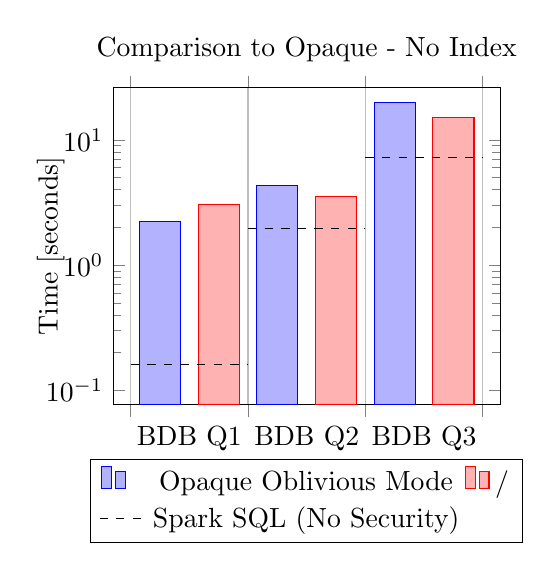
\begin{tikzpicture}
\centering
\begin{semilogyaxis}[
	log origin = infty,
	width=6.5cm,
	y label style={at={(axis description cs:-0.1,.5)},anchor=south},
	ytick={.1,1,10},
	ymin=.1,
	ylabel={Time [seconds]},
    title={Comparison to Opaque - No Index},
	symbolic x coords={BDB Q1, BDB Q2, BDB Q3, 4},
	x tick label style={
		/pgf/number format/1000 sep=},
	%%ylabel=Time (seconds),
	enlargelimits=0.05,
	legend style={at={(0.5,-0.17)},
	legend entries={Opaque Oblivious Mode, \name/, Spark SQL (No Security)},
	anchor=north,legend columns=2},
	ybar interval=.7,
    ]
%\addplot %baseline
%	coordinates {(BDB Q1, 54.18978) (BDB Q2, 205.78637) (BDB Q3, 131.29887) (4,1)};
\addplot %opaque obliv
	coordinates {(BDB Q1,2.2437) (BDB Q2,4.2908) (BDB Q3,19.9664) (4, 1)};
\addplot %us
	coordinates {(BDB Q1,3.03237) (BDB Q2, 3.5204) (BDB Q3,15.20425) (4,1)};
%\addplot %spark sql
%	coordinates {(BDB Q1,.1615) (BDB Q2,1.9757) (BDB Q3,7.2477) (4,1)}; 
    %\legend{Opaque Oblivious Mode,\name/, Spark SQL (No Security)}
    
\addlegendimage{line legend,black,sharp plot,dashed}
\coordinate (A) at (axis cs:BDB Q1,.1615);
\coordinate (B) at (axis cs:BDB Q2,.1615);
\coordinate (C) at (axis cs:BDB Q2,1.9757);
\coordinate (D) at (axis cs:BDB Q3,1.9757);
\coordinate (E) at (axis cs:BDB Q3,7.2477);
\coordinate (F) at (axis cs:4,7.2477);
 
\draw [black,sharp plot,dashed] (A) -- (B);
\draw [black,sharp plot,dashed] (C) -- (D);
\draw [black,sharp plot,dashed] (E) -- (F); 
    
\end{semilogyaxis}
\end{tikzpicture}
\vskip .3cm
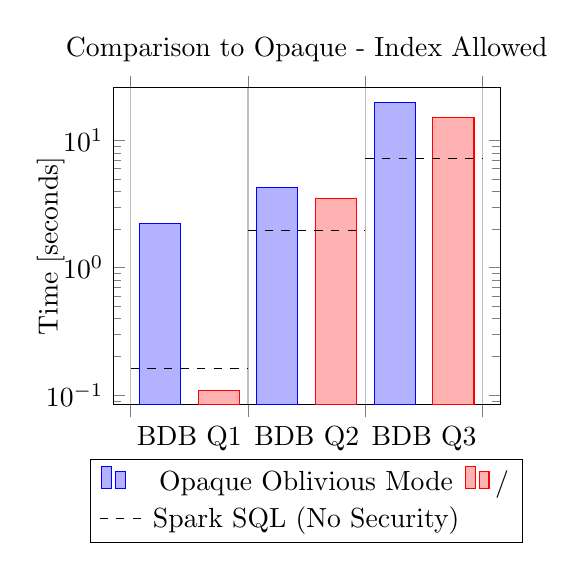
\begin{tikzpicture}
\centering
\begin{semilogyaxis}[
	log origin = infty,
	width=6.5cm,
	y label style={at={(axis description cs:-0.1,.5)},anchor=south},
	ylabel={Time [seconds]},
    title={Comparison to Opaque - Index Allowed},
	symbolic x coords={BDB Q1, BDB Q2, BDB Q3, 4},
	x tick label style={
		/pgf/number format/1000 sep=},
	%%ylabel=Time (seconds),
	enlargelimits=0.05,
	legend style={at={(0.5,-0.17)},
		legend entries={Opaque Oblivious Mode, \name/, Spark SQL (No Security)},
	anchor=north,legend columns=2},
	ybar interval=.7,
    ]
%\addplot %baseline
%	coordinates {(BDB Q1, 54.18978) (BDB Q2, 205.78637) (BDB Q3, 131.29887) (4,1)};
\addplot %opaque obliv
	coordinates {(BDB Q1,2.2437) (BDB Q2,4.2908) (BDB Q3,19.9664) (4, 1)};
\addplot %us
	coordinates {(BDB Q1,.10869) (BDB Q2, 3.5204) (BDB Q3,15.20425) (4,1)};
%\addplot %spark sql
%	coordinates {(BDB Q1,.1615) (BDB Q2,1.9757) (BDB Q3,7.2477) (4,1)};
    %\legend{Opaque Oblivious Mode,\name/, Spark SQL (No Security)}
    
    \addlegendimage{line legend,black,sharp plot,dashed}
\coordinate (A) at (axis cs:BDB Q1,.1615);
\coordinate (B) at (axis cs:BDB Q2,.1615);
\coordinate (C) at (axis cs:BDB Q2,1.9757);
\coordinate (D) at (axis cs:BDB Q3,1.9757);
\coordinate (E) at (axis cs:BDB Q3,7.2477);
\coordinate (F) at (axis cs:4,7.2477);
 
\draw [black,sharp plot,dashed] (A) -- (B);
\draw [black,sharp plot,dashed] (C) -- (D);
\draw [black,sharp plot,dashed] (E) -- (F); 
\end{semilogyaxis}
\end{tikzpicture}
\ignore{
\centering
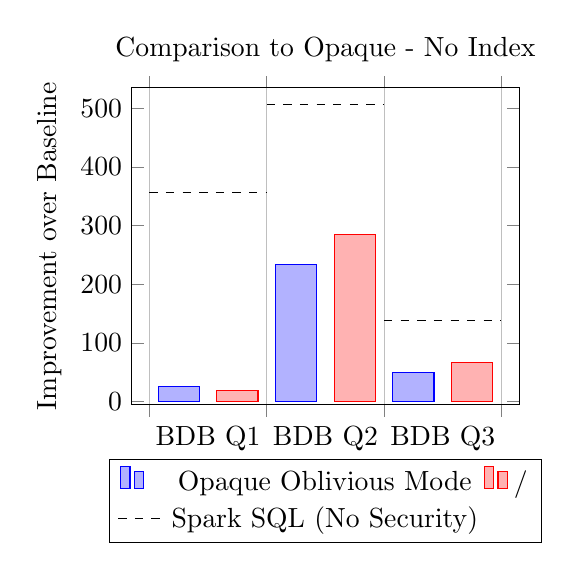
\begin{tikzpicture}
\begin{axis}[
	width=6.5cm,
	ylabel={Improvement over Baseline},
    title={Comparison to Opaque - No Index}, 
	symbolic x coords={BDB Q1, BDB Q2, BDB Q3, 4},
	ytick={0, 100, 200, 300, 400,500},
	%yticklabels={1$\times$, 10$\times$, 100$\times$, 500$\times$},
	x tick label style={
		/pgf/number format/1000 sep=},
	%%ylabel=Time (seconds),
	legend style={at={(0.5,-0.17)},
	legend entries={Opaque Oblivious Mode, \name/, Spark SQL (No Security)},
	anchor=north,legend columns=2},
	enlargelimits=0.05,
	ybar interval=0.7,
    ]
\addplot %opaque obliv
	coordinates {(BDB Q1,25.6) (BDB Q2,233.06) (BDB Q3,50.08) (4, 510)}; 
\addplot %us
	coordinates {(BDB Q1, 19) (BDB Q2, 284) (BDB Q3,65.8) (4,510)};
%\addplot %spark sql
%	coordinates {(BDB Q1,335.54) (BDB Q2,104.16) (BDB Q3,18.12) (4,1)};
\addlegendimage{line legend,black,sharp plot,dashed}
\coordinate (A) at (axis cs:BDB Q1,356.1);
\coordinate (B) at (axis cs:BDB Q2,356.1);
\coordinate (C) at (axis cs:BDB Q2,506.1);
\coordinate (D) at (axis cs:BDB Q3,506.1);
\coordinate (E) at (axis cs:BDB Q3,137.97);
\coordinate (F) at (axis cs:4,137.97);
 
\draw [black,sharp plot,dashed] (A) -- (B);
\draw [black,sharp plot,dashed] (C) -- (D);
\draw [black,sharp plot,dashed] (E) -- (F); 

%\legend{Opaque Oblivious, \name/, Spark SQL (No Security), NS}
\end{axis} 
\end{tikzpicture}
\vskip .3cm
\centering
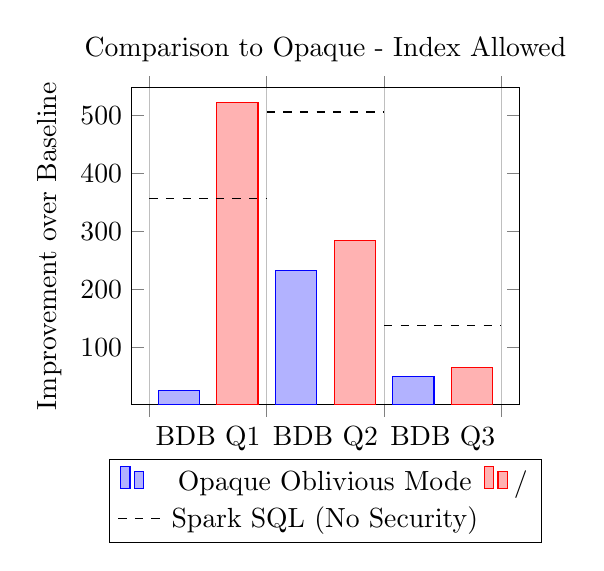
\begin{tikzpicture}
\begin{axis}[
	width=6.5cm,
	ylabel={Improvement over Baseline},
    title={Comparison to Opaque - Index Allowed}, 
	symbolic x coords={BDB Q1, BDB Q2, BDB Q3, 4},
	ytick={0, 100, 200, 300, 400,500},
	%ytick={30,100, 300,500},
	%yticklabels={30$\times$, 100$\times$, 500$\times$},
	x tick label style={
		/pgf/number format/1000 sep=},
	%%ylabel=Time (seconds),
	legend style={at={(0.5,-0.17)},
	legend entries={Opaque Oblivious Mode, \name/, Spark SQL (No Security)},
	anchor=north,legend columns=2},
	enlargelimits=0.05,
	ybar interval=0.7,
    ]
\addplot %opaque obliv
	coordinates {(BDB Q1,25.6) (BDB Q2,233.06) (BDB Q3,50.08) (4, 510)}; 
\addplot %us
	coordinates {(BDB Q1, 522.8) (BDB Q2, 284) (BDB Q3,65.8) (4,510)};
%\addplot %spark sql
%	coordinates {(BDB Q1,335.54) (BDB Q2,104.16) (BDB Q3,18.12) (4,1)};
\addlegendimage{line legend,black,sharp plot,dashed}
\coordinate (A) at (axis cs:BDB Q1,356.1);
\coordinate (B) at (axis cs:BDB Q2,356.1);
\coordinate (C) at (axis cs:BDB Q2,506.1);
\coordinate (D) at (axis cs:BDB Q3,506.1);
\coordinate (E) at (axis cs:BDB Q3,137.97);
\coordinate (F) at (axis cs:4,137.97);
 
\draw [black,sharp plot,dashed] (A) -- (B);
\draw [black,sharp plot,dashed] (C) -- (D);
\draw [black,sharp plot,dashed] (E) -- (F); 

%\legend{Opaque Oblivious, \name/, Spark SQL (No Security), NS}
\end{axis} 
\end{tikzpicture}
}
\caption{\name/ outperforms Opaque Oblivious~\cite{ZDB+17} by 1.2-20$\times$ and never runs more than 2.1$\times$ slower than Spark SQL~\cite{SparkSQL} on the Q1-Q3 of the Big Data Benchmark~\cite{BDB}. Even without use of an index, \name/ performs comparably to Opaque Oblivious.} 
\label{figOpaque} 
\end{figure} 

Figure~\ref{figOpaque} compares \name/ with Opaque's oblivious mode~\cite{ZDB+17} and Spark SQL~\cite{SparkSQL} on the first three queries of the Big Data Benchmark~\cite{BDB} on tables of 360,000 and 350,000 rows. We omit the benchmark's fourth query as neither \name/ nor Opaque support the external scripts needed for it. Opaque, like \name/, centers its design on a secure SGX enclave and can be configured in either an ``encryption'' mode, which leaks access patterns but offers performance close to Spark SQL and an ``oblivious'' mode that hides access patterns to data by making sure to fit sensitive memory accesses inside the trusted enclave memory and achieving a security level similar to ours, albeit by very different means. Spark SQL provides no security guarantees and provides a measure of the performance achievable without any security concerns. Both Opaque and Spark SQL are run in a single node configuration on our device. 

\name/, when allowed to use indexes, outperforms Opaque on all three BDB queries, ranging from 1.2$\times$ speedup on query 2 to 20$\times$ speedup on query 1. The strong performance of \name/ compared to Opaque and Spark SQL on query 1 is due to \name/'s oblivious index, which allows it to only examine a small portion of the table whereas Opaque and Spark SQL, which aim to primarily handle analytic workloads, scan the entire table to satisfy the query. Even without using an index to speed up query 1, \name/ performs comparably to Opaque. Moreover, for queries 2 and 3, although \name/ is slower than Spark SQL, it is only 1.8$\times$ slower on query 2 and 2.1$\times$ slower on query 3, putting \name/ safely in the realm of tools whose performance is practical for real applications. 

\subsection{Comparison to Sophos}
\begin{figure}
\small
\centering
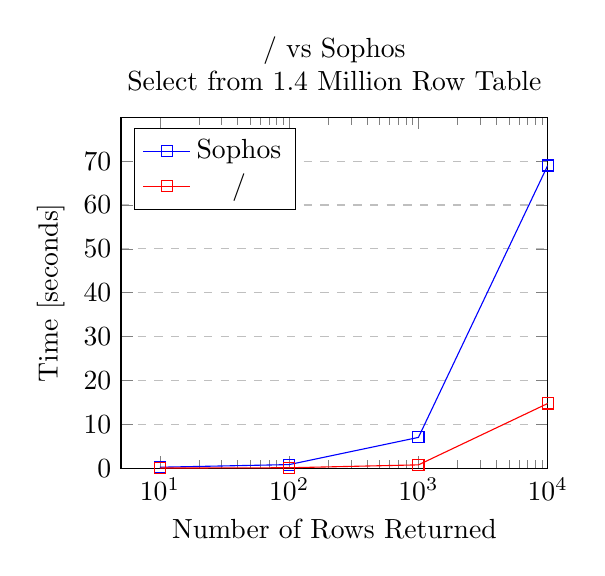
\begin{tikzpicture}
\begin{semilogxaxis}[
    title style={align=center}, title={\name/ vs Sophos\\Select from 1.4 Million Row Table},
    width=7cm,
    xlabel={Number of Rows Returned},
    ylabel={Time [seconds]},
    xmin=5, xmax=10000,
    ymin=0, ymax=80,
    xtick={10,100,1000,10000},
    ytick={0,10,20,30,40,50,60,70},
    legend pos=north west,
    ymajorgrids=true,
    grid style=dashed,
    ]
    \addplot[
    color=blue,
    mark=square,
    ]
    coordinates {
    (10,.2)(100,.8)(1000,7)(10000,69)
    };
    \addplot[
    color=red,
    mark=square,
    ]
    coordinates {
    (10,.01053)(100,.07797)(1000,.73794)(10000,14.73558)
    };
    \legend{Sophos, \name/}
\end{semilogxaxis}
\end{tikzpicture}
\caption{Comparison of \name/ to Sophos SSE scheme\cite{Bost16} on 1.4 million rows of data. \name/ outperforms Sophos by 19$\times$ when selecting 10 rows and by 4.7$\times$ when selecting 10,000 rows. Unlike \name/, Sophos does not use SGX but leaks access patterns to data.\ignore{make sure to mention in text that sophos numbers come from original paper and were gathered on a much more powerful computer and also used multithreading. Also, if we extrapolate the numbers to 100k rows retrieved, \name/ linear scan actual beats both \name/ index and sophos}} 
\label{figSophos}
\end{figure}

We compare the performance of \name/'s oblivious index to the searchable symmetric encryption (SSE) scheme Sophos~\cite{Bost16} in Figure~\ref{figSophos}. Sophos does not provide obliviousness guarantees, meaning it leaks access patterns to rows in a table, and it does not use hardware enclaves to achieve security. It does, however, offer a ``forward-secrecy'' property not found in many SSE schemes. As such, it provides a good point of comparison for the performance of our SGX-based oblivious Indexed tables with a non-SGX based, non-oblivious index that still provides reasonable privacy guarantees. Sophos only provides the ability to search for exact keyword matches via an inverted index, so we compare on simulated data. Specifically, we compare against the performance numbers reported in the original Sophos paper for a table of 1.4 million rows and measured using a much more powerful machine than ours: an Intel Core i7 4790K 4.00GHz CPU with 8 logical cores, 16GB of RAM, a 250 GB Samsung 850 EVO SSD, running on OS X.10. Despite the difference in hardware and the fact that the Sophos implementation is multithreaded, \name/ outperforms Sophos by 4.7-19$\times$ depending on the size of the number of rows returned by a query. We observe that the performance tipping point between Indexed and Linear tables in \name/ arrives between the $10^4$ and $10^5$ rows returned marks in this experiment, and \name/'s performance on larger queries beyond that point would remain constant. 

\subsection{Padding Mode Overhead}
\begin{figure}
\small
\centering
\begin{tabular}{llll}
\textbf{Query Type} & \textbf{No Padding} & \textbf{Padding} & \textbf{Slowdown} \\\hline
Aggregate & 0.72s & 7.31s & 10.2$\times$\\
Select (Linear) & 1.40s & 8.12s & 5.8$\times$\\
Select (Index) & 0.63s & 2.35s & 3.7$\times$\\
Insert (Index) & 0.20s & 0.25s & 1.3$\times$\\
Delete (Index) & 0.43s & 0.49s & 1.1$\times$\\
\end{tabular}
\caption{Slowdown of \name/ in padding mode for queries in the CFPB table of 107,000 rows padded to 500,000 rows.}
\label{figPad}
\end{figure}

In Figure~\ref{figPad}, we report on the overhead of using padding mode in \name/ to hide not only access patterns to data but also all information regarding the sizes of tables, whether they be at rest in the database, intermediate tables constructed in handling a query, or the results returned from a query. The table shows query results for the 107,000 row CFPB table padded up to 500,000 rows. 

Opaque~\cite{ZDB+17} describes an oblivious pad mode, but this mode remains unimplemented. To our knowledge, no other comparable system exists with an implemented oblivious padding mode, so we are unable to compare our padding performance to prior work. The results do, however, represent reasonable slowdowns for inflating the size of a table by approximately 5$\times$. 

\subsection{Microbenchmarks}
\begin{figure*}
\small
\centering
\begin{tabular}{@{}l@{}l@{}l}
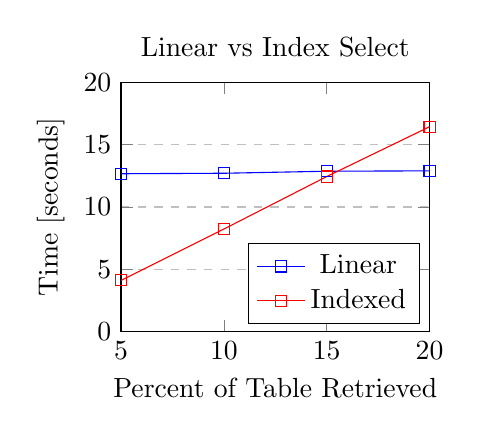
\begin{tikzpicture}
\begin{axis}[
    title={Linear vs Index Select},
    	width=5.5cm,
    xlabel={Percent of Table Retrieved},
    ylabel={Time [seconds]},
    xmin=5, xmax=20,
    ymin=0, ymax=20,
    xtick={5, 10, 15, 20},
    ytick={0,5,10,15,20},
    legend pos=south east,
    ymajorgrids=true,
    grid style=dashed,
    ]
    \addplot[
    color=blue,
    mark=square,
    ]
    coordinates {
    (5,12.67146)(10,12.71014)(15,12.87276)(20,12.90335)
    };
    \addplot[
    color=red,
    mark=square,
    ]
    coordinates {
    (5,4.10491)(10,8.22869)(15,12.44472)(20,16.44773)
    };
    \legend{Linear, Indexed}
\end{axis}
\end{tikzpicture}

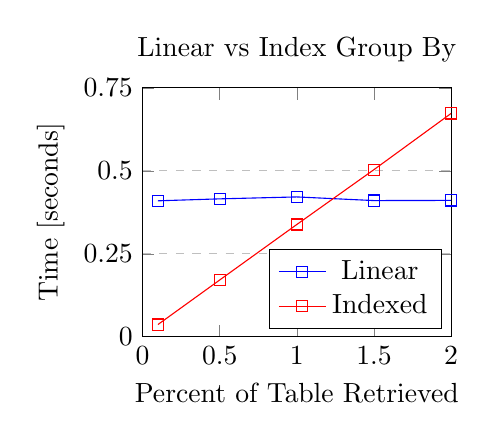
\begin{tikzpicture}
\begin{axis}[
    title={Linear vs Index Group By},
        ylabel={Time [seconds]},
        	width=5.5cm,
    xlabel={Percent of Table Retrieved},
    xmin=0, xmax=2,
    ymin=0, ymax=.75,
    xtick={0,.5,1,1.5,2},
    ytick={0,.25,.5,.75,1},
    legend pos=south east,
    ymajorgrids=true,
    grid style=dashed,
    ]
    \addplot[
    color=blue,
    mark=square,
    ]
    coordinates {
    (.1,.40982)(.5,.41572)(1,.42153)(1.5,.41053)(2,.41103)
    };
    \addplot[
    color=red,
    mark=square,
    ]
    coordinates {
    (.1,.03718)(.5,.17128)(1,.33852)(1.5,.50370)(2,.67299)
    };
    \legend{Linear, Indexed}
\end{axis}
\end{tikzpicture}
&
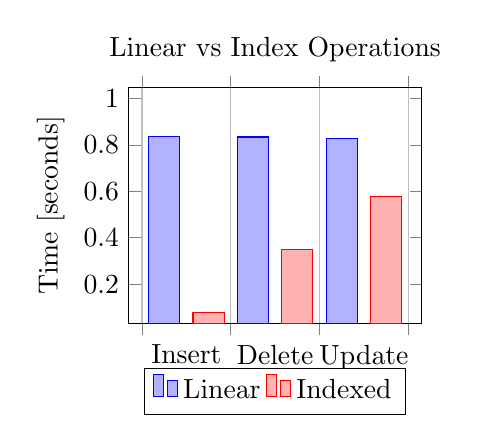
\begin{tikzpicture}
\begin{axis}[
	width=5.3cm,
    title={Linear vs Index Operations},
        ylabel={Time [seconds]},
	symbolic x coords={Insert, Delete, Update, 4},
	x tick label style={
		/pgf/number format/1000 sep=},
	%%ylabel=Time (seconds),
	enlargelimits=0.05,
	legend style={at={(0.5,-0.19)},
	anchor=north,legend columns=-1},
	ybar interval=0.7,
    ]
\addplot 
	coordinates {(Insert,.83527) (Delete,.83431) (Update,.82696) (4, 1)};
\addplot
	coordinates {(Insert,.0772) (Delete,.35019) (Update,.57801) (4,1)};
    \legend{Linear, Indexed}
\end{axis}
\end{tikzpicture}\\
\end{tabular}
\caption{Comparison of Linear and Index versions of operators over 100,000 rows of fabricated data. Linear scans do better when most of the data needs to be accessed, but Indexed structures perform far better for small queries. Operations involving modification of the database are far faster for indexed structures.}
\label{figC1}
\end{figure*}

\begin{figure}
\small
\centering
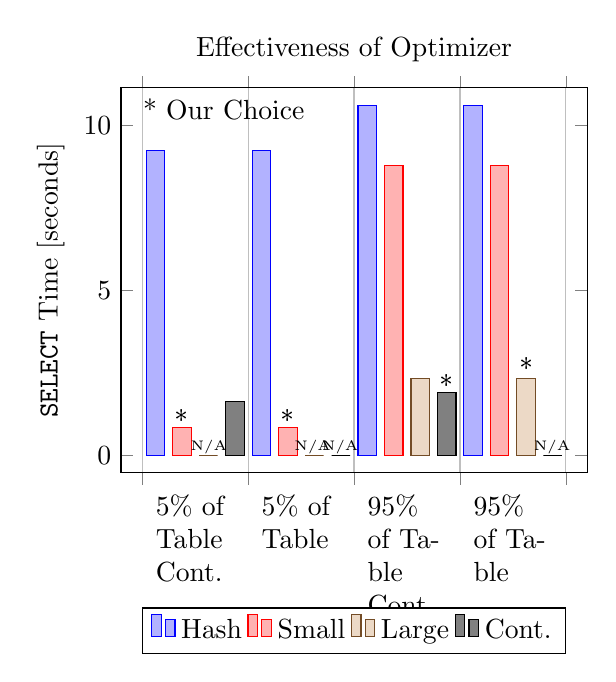
\begin{tikzpicture}
\centering
\begin{axis}[
	width=7.5cm,
	ybar interval=.7,
	ylabel={\texttt{SELECT} Time [seconds]},
    title={Effectiveness of Optimizer}, 
	symbolic x coords={5\% of Table Cont., 5\% of Table, 95\% of Table Cont., 95\% of Table, 4},
	legend style={at={(0.5,-0.35)},
	anchor=north,legend columns=4},
	xtick=data,
	x tick label style={text width=1cm},
	%%ylabel=Time (seconds),
	enlargelimits=0.05,
    ]
	
\addplot 
	coordinates {(5\% of Table Cont., 9.24) (5\% of Table, 9.24) (95\% of Table Cont., 10.6) (95\% of Table, 10.6) (4,1)}; %hash
\addplot 
	coordinates {(5\% of Table Cont., .84) (5\% of Table, .84) (95\% of Table Cont., 8.77) (95\% of Table, 8.77) (4,1)};	%small
	\addplot 
	coordinates {(5\% of Table Cont., 0) (5\% of Table, 0) (95\% of Table Cont., 2.33) (95\% of Table, 2.33) (4,1)};	%large
\addplot 
	coordinates {(5\% of Table Cont., 1.63) (5\% of Table, 0) (95\% of Table Cont., 1.89) (95\% of Table, 0) (4,1)};	%cont

\legend{Hash, Small, Large, Cont.}
       \draw (37,12) node {\textasteriskcentered}; 
       \draw (77,105) node {* Our Choice}; 
       \draw (137,12) node {\textasteriskcentered}; 
       \draw (287,22.5) node {\textasteriskcentered}; 
       \draw (362.5,27.5) node {\textasteriskcentered}; 
       \draw (63,2.5) node {\tiny{N/A}}; 
       \draw (161,2.5) node {\tiny{N/A}}; 
       \draw (187,2.5) node {\tiny{N/A}}; 
       \draw (387,2.5) node {\tiny{N/A}}; 
       
\end{axis}
\end{tikzpicture}
\caption{Our optimizer picks the best algorithm for handling \texttt{SELECT} queries based on a preliminary scan that determines whether the data to be returned is small, large, or consists of a continuous set of rows in the table.} 
\label{figC3}
\end{figure}
\noindent \textbf{Comparison of Linear and Indexed tables}.
By providing both Indexed and Linear tables and optimizing queries based on information gained through a first pass over the data, \name/ to makes meaningful performance improvements for diverse queries. To this end, Figure~\ref{figC1} compares the performance of Linear and Indexed tables on \texttt{SELECT} (hash algorithm), \texttt{GROUP BY} (low-cardinality), \texttt{INSERT}, \texttt{DELETE}, and \texttt{UPDATE} queries. Linear scans perform better as the amount of data retrieved from a table increases since the cost of the scan is amortized over more rows, but smaller queries perform significantly better using an index. This finding contrasts claims in prior work~\cite{RLT15} that indicate linear scans always perform better than ORAM for oblivious memory access. In general, Indexed \texttt{INSERT}, \texttt{DELETE}, and \texttt{UPDATE} queries significantly outperform Linear tables. Indexed insertions complete faster than deletions and updates because insertions only need to find a place in the B+ tree, but deletions and updates need to scan forward from that point to find rows that need to be deleted/updated.

\noindent \textbf{Effectiveness of Optimizer}. 
Figure~\ref{figC3} demonstrates the effectiveness of \name/'s choice of \texttt{SELECT} algorithms, comparing our various algorithms on queries that retrieve 5\% and 95\% percent of a fabricated 100,000 row table. Although the ``Hash'' algorithm performs the best asymptotically, the figure demonstrates that knowledge gleaned only from \name/'s intended leakage about the results of a query (whether it is small/large or a continuous set of rows) suffices to pick an algorithm that will perform much better in practice. Equally impressive gains appear in the choice of \texttt{GROUP BY} algorithm for real queries: the high-cardinality aggregation algorithm used for the query on the USERVISITS table (shown in Figure~\ref{figQueries}) performs 58$\times$ better than the low-cardinality algorithm would on the same query. 

\section{Related Work}\label{related}

\name/ is related to a number of prior works involving cryptographically-protected databases and applications of trusted hardware.

  \noindent \textbf{Cryptographically-protected database search}. 
A testament to the importance of the problem of search over encrypted data in databases lies in the extensive prior work on the subject, summarized and systematized by Fuller et al~\cite{FVY+17}. Perhaps the most widely known work in this area is CryptDB~\cite{PRZB12}, which implements a tradeoff between security and performance by encrypting each field in a table according to the type of operation expected to be used on the data in that field. Arx~\cite{PBP16}, a more recent system, keeps all data encrypted at the highest level of security and makes clever use of data structures to allow for efficient operations over data. Another common class of solutions are those which use an inverted index to allow searches on stored encrypted data, as exemplified by Demertzis et al~\cite{DPP+16}. These schemes rely on searchable symmetric encryption (SSE) as a primitive, a recent example of which is Sophos~\cite{Bost16}, which boasts forward security -- queries authorized in the past do not leak any new information when additional documents are added to an existing database. A very recent follow-up work to Sophos introduces a notion of backward-security and provides improved constructions \cite{BMO17}. 

The diversity of security goals and varied use cases for which cryptographically protected databases have been designed have led to a plague of attacks which show that real-world applications of schemes proven secure in theoretical models can in fact leak far more data than would be expected from an initial examination of a system's security properties. Initiated by Islam et al~\cite{IKK12} and continuing with improved results such as those of Naveed et al~\cite{NKW15} and Cash et al~\cite{CGPR15} to name only a few, such attacks show that inference from known context of the data used, additional correlated public data, or even just the leakage inherent in a scheme itself, can be used to attack various schemes in ways not anticipated in their original security models. Zhang et al~\cite{ZKP16} show that even schemes with very little leakage are susceptible to attack. In hiding even the access patterns to data in our solution, we hope to minimize the extent to which \name/ is vulnerable to such techniques.   

  \noindent \textbf{Trusted hardware}. 
Trusted hardware can be used to achieve security properties that are difficult, impractical, or potentially impossible with traditional cryptographic assumptions. For example, a number of hardware or hardware/software based solutions exist with the explicit goal of rendering programs' memory traces oblivious~\cite{CLD16, LHM+15, MLS+13}. Intel SGX, on which we will focus, has been used to implement practical functional encryption~\cite{FVBG16} and obfuscation~\cite{NFR+17}, both functionalities which can currently only be constructed using heavy cryptographic machinery.

In recent years, a number of generic tools have been designed to provide legacy applications the heightened security available from SGX. Haven~\cite{BPH15} shields execution of legacy programs from a malicious OS. Panoply and SCONE~\cite{STTS17, ATG+16} provide SGX-protected Linux OS and container abstractions. In the distributed setting, Ryoan~\cite{HZX+16} is a sandbox for computation on secret data. 

In addition to general tools, applications to securely conduct data analytics or handle data in the cloud represent a compelling practical use case for SGX hardware. In this vein, many works implement variations of existing tools and services rendered secure via SGX. M2R~\cite{DSC+15} and VC3~\cite{SCF+15} provide MapReduce and cloud data analytics functionalities, respectively, and Opaque~\cite{ZDB+17} provides secure support for Spark SQL. SecureKeeper~\cite{BWG+16} uses SGX to build a confidential version of Apache's ZooKeeper (\url{zookeeper.apache.org}). More fundamental primitives for databases and oblivious computation in general are provided by HardIDX~\cite{FBB+17}, a database index in SGX, and ZeroTrace~\cite{SGF17} which provides oblivious memory primitives based on ORAM as well as an analysis of parameter optimizations for using an ORAM controller in SGX for data storage. None of the solutions above, with the exception of ZeroTrace, use ORAM to hide memory access patterns. Instead, they either make use of memory-oblivious algorithms suited to the tasks they undertake or remain vulnerable to side-channel attacks targeting memory access patterns. 

Trusted hardware assumption like those underlying SGX fundamentally differ from traditional mathematical assumptions in that, whereas the validity of a mathematical assumption cannot be challenged by the vicissitudes of succeeding implementations, attacks, and side-channels, the legitimacy of a hardware assumption relies directly on the ability of a piece of manufactured hardware to repel practical attacks. As such, the SGX literature includes a number of works that aim to reveal practical side channels in the implementation of SGX and develop techniques to obviate the risks presented by each known family of attacks. Xu et al~\cite{XCP15} use page faults and other ``controlled channel'' side channels to extract images and text documents from protected memory, and Lee et al~\cite{LSG+16} use the fact that SGX does not clear branch history when leaving an enclave to infer details of branches taken in protected code. In the multithreaded regime, Weichbrodt et al~\cite{WKPK16} compromise security by leveraging synchronization bugs. Defenses against such attacks include the work of Shinde et al~\cite{SCNS16} and Raccoon~\cite{RLT15} which close side channels by making the memory trace of a program oblivious or obfuscated. SGX-Shield~\cite{SLK+17} enables address space layout randomization for SGX, and, finally, T-SGX~\cite{SLKP17} protects against side-channel attacks by using another set of hardware features, Transactional Synchronization Extensions (TSX) to close side channels that could otherwise be exploited by a malicious OS. \name/ can be generically combined with any of these solutions to provide higher levels of confidence in the security of the enclave.  

\section{Conclusion}\label{conclusion}
We have presented \name/, a cryptographically-protected database system based on Intel SGX that leaks only table sizes and its query plan (and additionally offers a padding mode to hide even table sizes). We have shown that \name/ handles practical data sets with performance surpassing prior work with similar security properties as well as other existing solutions with more permissive leakage functions. It is our hope that solutions like \name/ based on SGX and other techniques that leverage hardware-based advantages can enable rapid advances in the performance and security of solutions to difficult problems related to private databases and search over encrypted data. 

%\section*{Acknowledgements}

{\footnotesize \bibliographystyle{acm}
\bibliography{oramsgx}}
 

%\theendnotes

\end{document}




